%!TEX root = ../Thesis.tex
%!TEX program = xelatex
\documentclass[../Thesis]{subfiles}

% 本文
\begin{document}
\chapter{実験}
\section{実験環境}
本研究における実験環境を\tref{tab03}に示す.

\begin{table}[tbp]
  \centering
	\caption{実験環境}
	\label{tab03}
	\begin{tabular}{l l}
		\hline
		CPU & Intel® Core™ i7-7500U \\
		メモリ & 8.00 GB \\
		OS & Windows 10 Pro \\
		使用言語 & Python 3.8.0 \\
		使用ライブラリ & OpenCV 4.2.0 \\ \hline
	\end{tabular}
\end{table}

\section{使用データ}
本研究では国土地理院提供の平成29年7月九州北部豪雨のドローン空撮映像\cite{web02}を用いた.空撮映像の詳細を\tref{tab04}と\tref{tab05}に示す.

\begin{table}[tbp]
	\centering
	\caption{使用データ(実験1)}
	\label{tab04}
	\begin{tabular}{l l}
		\hline
		災害名称 & 平成29年7月九州北部豪雨 \\
		撮影箇所 & 福岡県朝倉市赤谷川 \\
		撮影日時 & 平成29年7月7日15時30分 \\
		解像度 & 1920 × 1080 画素 \\
		提供 & 国土交通省国土地理院 \\ \hline
	\end{tabular}
\end{table}

\begin{table}[tbp]
	\centering
	\caption{使用データ(実験2)}
	\label{tab05}
	\begin{tabular}{l l}
		\hline
		災害名称 & 平成29年7月九州北部豪雨 \\
		撮影箇所 & 福岡県朝倉市奈良ヶ谷 \\
		撮影日時 & 平成29年7月7日17時45分 \\
		解像度 & 1440 × 1080 画素 \\
		提供 & 国土交通省国土地理院 \\ \hline
	\end{tabular}
\end{table}


\section{実験結果}
\subsection{入力画像}
実験に使用したドローン空撮映像から切り取ったフレーム画像を\fref{img06}と\fref{img07}に示す.

\begin{figure}[tbp]
	\centering
	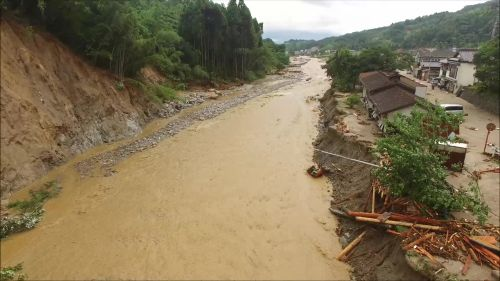
\includegraphics[width=12cm]{img/original1.png}
	\caption{入力画像(実験1)}
	\label{img06}
\end{figure}

\begin{figure}[tbp]
	\centering
	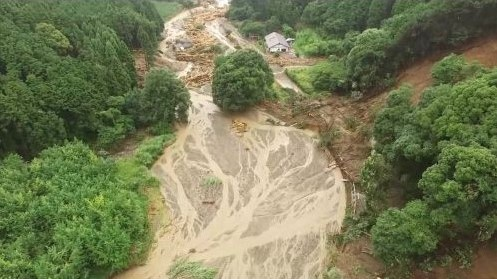
\includegraphics[width=12cm]{img/original2.png}
	\caption{入力画像(実験2)}
	\label{img07}
\end{figure}


\subsection{領域分割}
前節の入力画像をMean-Shift法にて領域分割した結果を\fref{img08}と\fref{img09}に示す.

\begin{figure}[tbp]
	\centering
	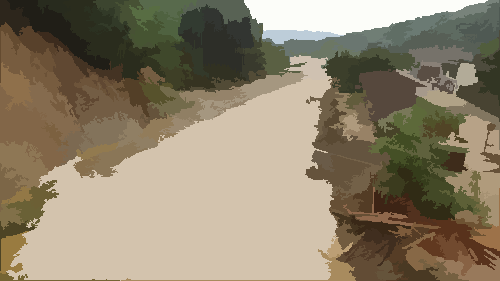
\includegraphics[width=12cm]{img/meanshift1.png}
	\caption{領域分割結果(実験1)}
	\label{img08}
\end{figure}
\begin{figure}[tbp]
	\centering
	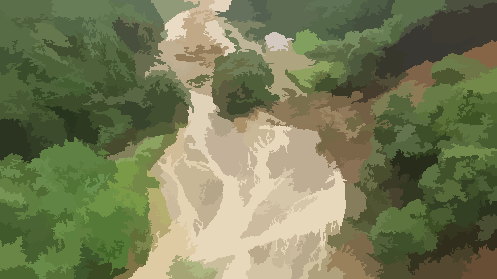
\includegraphics[width=12cm]{img/meanshift2.png}
	\caption{領域分割結果(実験2)}
	\label{img09}
\end{figure}


\subsection{ヒストグラム均一化}
領域分割を適用した画像にCLAHEのアルゴリズムにてヒストグラム均一化を行った結果を\fref{img10}と\fref{img11}に示す.

\begin{figure}[tbp]
	\centering
	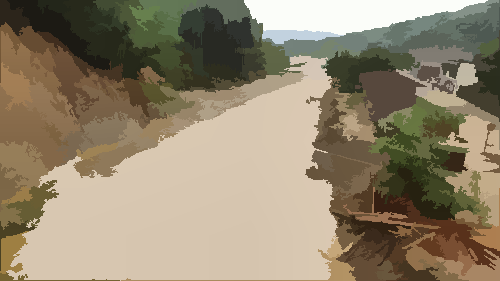
\includegraphics[width=12cm]{img/equalization1.png}
	\caption{ヒストグラム均一化結果(実験1)}
	\label{img10}
\end{figure}
\begin{figure}[tbp]
	\centering
	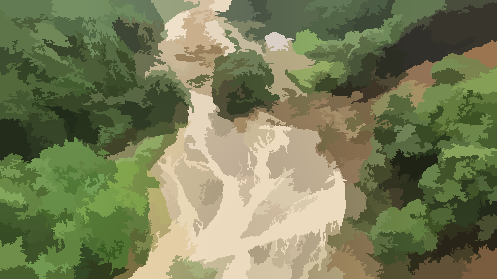
\includegraphics[width=12cm]{img/equalization2.png}
	\caption{ヒストグラム均一化結果(実験2)}
	\label{img11}
\end{figure}

\subsection{災害領域検出}
\label{detection}
ヒストグラム均一化を適用した画像に対し閾値処理にて災害領域である斜面崩壊・浸水領域を検出した結果を\fref{img12}と\fref{img13}に示す.なお,赤は斜面崩壊,黄は浸水領域を表す.

\begin{figure}[tbp]
	\centering
	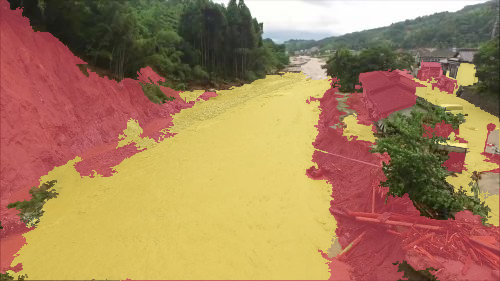
\includegraphics[width=12cm]{img/detection1.png}
	\caption{災害領域検出(実験1)}
	% \caption{斜面崩壊領域検出(実験1)}
	\label{img12}
\end{figure}
\begin{figure}[tbp]
	\centering
	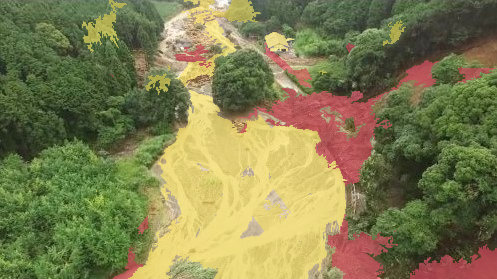
\includegraphics[width=12cm]{img/detection2.png}
	\caption{災害領域検出(実験2)}
	\label{img13}
\end{figure}

\subsection{不要領域除去}
\label{rejection}
ヒストグラム均一化を適用した画像に対し閾値処理にて不要領域である植生・空・瓦礫・建物領域を検出した結果を\fref{img14}と\fref{img15}に示す.なお,青は空,緑は植生,橙は瓦礫,紫は建物領域を表す.

\begin{figure}[tbp]
	\centering
	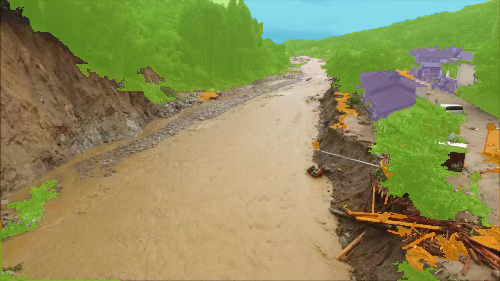
\includegraphics[width=12cm]{img/rejection1.png}
	\caption{不要領域検出(実験1)}
	\label{img14}
\end{figure}
\begin{figure}[tbp]
	\centering
	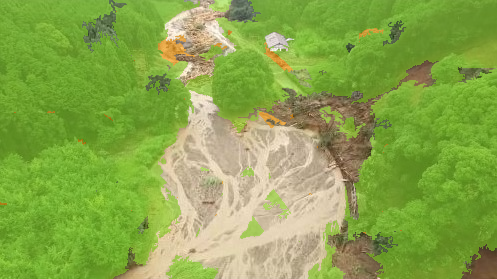
\includegraphics[width=12cm]{img/rejection2.png}
	\caption{不要領域検出(実験2)}
	\label{img15}
\end{figure}

\subsection{統合処理}
	\ref{detection}項にて検出した領域から\ref{rejection}項にて検出した領域を除去し,最終出力結果とする.最終的に斜面崩壊・浸水領域を検出した結果を\fref{img16}と\fref{img17}に示す.なお,赤は斜面崩壊,黄は浸水領域を表す.

\begin{figure}[tbp]
	\centering
	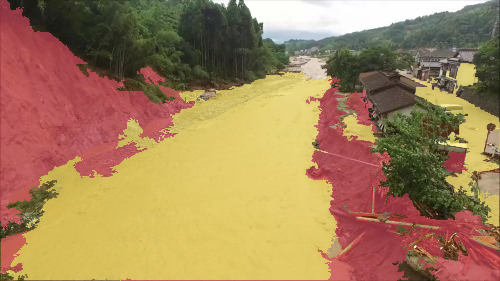
\includegraphics[width=12cm]{img/result1.png}
	\caption{最終出力結果(実験1)}
	\label{img16}
\end{figure}
\begin{figure}[tbp]
	\centering
	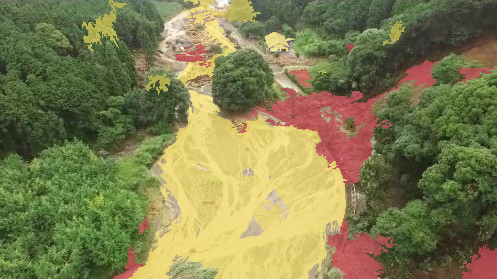
\includegraphics[width=12cm]{img/result2.png}
	\caption{最終出力結果(実験2)}
	\label{img17}
\end{figure}

\section{精度評価}
目視判読による斜面崩壊・浸水領域の正解データを手動で作成し,画素単位で判定を行った結果から適合率(precision),再現率(recall),F値(F-measure)をそれぞれ算出した.適合率,再現率,F値の概念図を\fref{img18}に,導出式を\Fref{form12}--\Fref{form14}に示す.TP(True Positive)は正しく検出した画素,FP(False Positive)は誤検出した画素,FN(False Negative)は未検出の画素,TN(True Negative)は非検出画素を正しく未検出とした画素を表す.また,適合率は検出画素全体における正解画素の割合,再現率は正解画素全体における検出画素の割合,F値は適合率と再現率の調和平均で表した指標である.なお,F値が高いほど精度が高いことを表す.最後に,本研究にて正解画像として作成した画像を\fref{img19}と\fref{img20}に,本手法と先行研究の精度評価結果を\tref{tab06}に示す.

\begin{figure}[tbp]
	\centering
	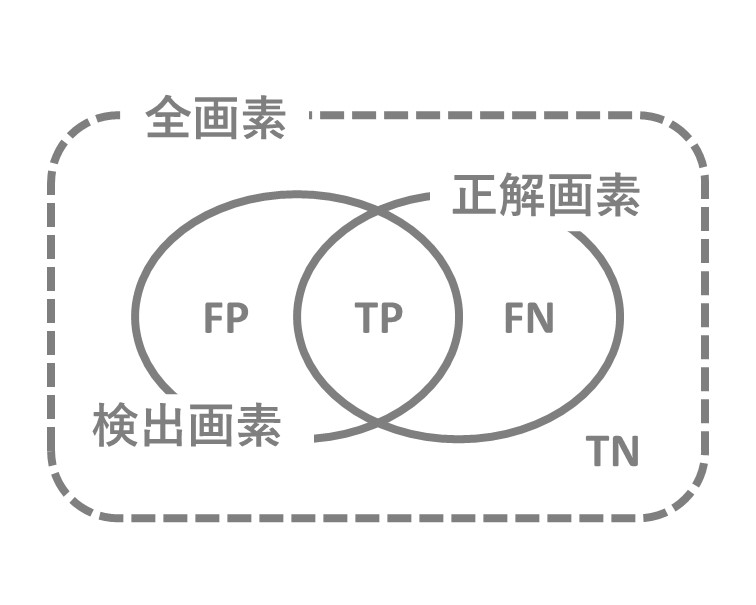
\includegraphics[width=12cm]{img/evaluation.jpg}
	\caption{精度評価概念図}
	\label{img18}
\end{figure}

\begin{equation}
  \begin{array}{l}
  	{\rm precision} = \cfrac{{\rm TP}}{{\rm TP}+{\rm FP}} \\
  \end{array}
\label{form12}
\end{equation}
\begin{equation}
  \begin{array}{l}
  	{\rm recall} = \cfrac{{\rm TP}}{{\rm TP}+{\rm FN}} \\
  \end{array}
\label{form13}
\end{equation}
\begin{equation}
  \begin{array}{l}
  	{\rm F\mathchar`-measure} = 2 \times \cfrac{{\rm recall} \times {\rm precision}}{{\rm recall}+{\rm precision}}
  \end{array}
\label{form14}
\end{equation}

\begin{figure}[tbp]
	\centering
	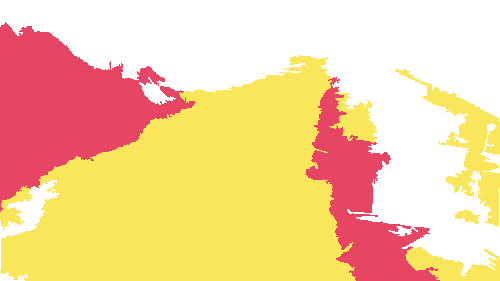
\includegraphics[width=12cm]{img/answer1.png}
	\caption{正解画像(実験1)}
	\label{img19}
\end{figure}
\begin{figure}[tbp]
	\centering
	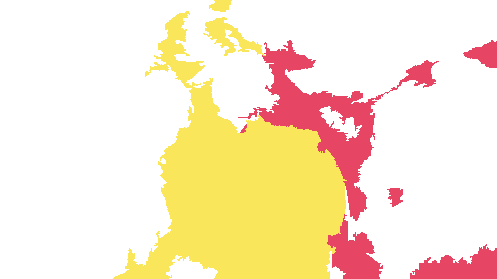
\includegraphics[width=12cm]{img/answer2.png}
	\caption{正解画像(実験2)}
	\label{img20}
\end{figure}

\begin{table}[tbp]
	\centering
	\caption{精度評価}
	\label{tab06}
	\begin{tabular}{c c c c c c}
		\hline
		手法 & 領域 & 実験 & 適合率 & 再現率 & F値 \\
		\hline
		\hline
		提案手法 & 斜面崩壊 & 実験1 & 0.596 & 0.953 & 0.733 \\
		提案手法 & 斜面崩壊 & 実験2 & 0.653 & 0.754 & 0.700 \\
		提案手法 & 浸水 & 実験1 & 0.987 & 0.848 & 0.912 \\
		提案手法 & 浸水 & 実験2 & 0.900 & 0.826 & 0.861 \\
		\hline
		中山らの手法 & 斜面崩壊 & 実験1 & 0.640 & 0.770 & 0.700 \\
		中山らの手法 & 斜面崩壊 & 実験2 & 0.620 & 0.720 & 0.660 \\
		雨宮らの手法 & 浸水 & 実験1 & 0.748 & 0.899 & 0.817 \\
		雨宮らの手法 & 浸水 & 実験2 & 0.719 & 0.722 & 0.720 \\
		\hline
	\end{tabular}
\end{table}


\section{考察}
\subsection{精度評価について}
平成29年7月九州北部豪雨の被災箇所である2地区の空撮画像を用いて実験を行った結果,斜面崩壊・浸水領域のF値のどちらも70\%以上を達成した.\tref{tab06}より全てのF値において先行研究と同等の精度で災害領域の検出に成功した.よって,災害時の観測手段としてドローンの有効性を精度の面で示すことができた.しかし,適合率と再現率において先行研究よりも検出精度が低くなった実験が存在した.特に斜面崩壊領域の適合率と浸水領域の再現率が先行研究より低い精度となった.これには以下の理由が考えられる. \\
\quad まず,斜面崩壊領域検出に関し,色相が類似している瓦礫・建物領域の誤検出が考えられる.瓦礫領域についてはエッジ抽出率にて検出を行っており,閾値を低く設定したため十分に除去ができず,誤検出が多くなったと推察される.しかし,斜面崩壊領域はエッジが多いという特徴があり,エッジ抽出率の閾値が高いと斜面崩壊領域が除去されるため,トレードオフの関係であると考えられる. \\
\quad 次に,斜面崩壊と浸水領域同士の誤検出が考えられる.どちらも閾値処理の際に色相,彩度,輝度を用いており,斜面崩壊領域であれば彩度が高く,輝度が低いといった特徴がある.しかし,画像中の領域ごとに光量や影の有無が異なるため,輝度などの指標による閾値処理が失敗する領域が存在すると考えられる. \\

% \begin{table}[tbp]
% 	\centering
% 	\caption{先行研究における精度評価}
% 	\label{tab07}
% 	\begin{tabular}{l l l l l l}
% 		\hline
% 		手法 & 領域 & 実験 & 適合率 & 再現率 & F値 \\
% 		\hline
% 		\hline
% 		中山らの手法 & 斜面崩壊 & 実験1 & 0.640 & 0.770 & 0.700 \\
% 		中山らの手法 & 斜面崩壊 & 実験2 & 0.620 & 0.720 & 0.660 \\
% 		雨宮らの手法 & 浸水 & 実験1 & 0.748 & 0.899 & 0.817 \\
% 		雨宮らの手法 & 浸水 & 実験2 & 0.719 & 0.722 & 0.720 \\
% 		\hline
% 	\end{tabular}
% \end{table}

\subsection{建物領域検出について}
実験1,2においてF値は先行研究と同等の精度を達成したが,先行研究で問題になっていた山間部での建物領域は実験2において検出に失敗した.GSIは本来,衛星画像にて裸地を示す指標であり,ドローンのような高解像度画像に用いる指標ではない点が考えられる.建物領域検出においてGSIを使用したが,GSI値が大きいほど裸地に近いことを示す.つまり,土が露出している裸地とは逆に,表面が滑らかである建物領域はGSI値が小さいと考え本指標を用いたが,ドローンは高解像度な映像による細かいテクスチャが判別できるため,衛星画像による指標をドローン空撮画像に適用することは適切でないと推測される. \\

% DEMと光学衛星、光学衛星と補助は難易度張り違う、位置合わせ
% 直下視点

% \subsection{ドローンの有効性について}



\end{document}
